A partir do problema identificado e da revisão da literatura foi encontrado
que o desenvolvimento de ontologias é um área de pesquisa abrangida
pela Web Semântica que permite desenvolver sistemas web baseados em
conhecimento, satisfazendo os requisitos de desenvolvimento do SAD
SustenAgro explicados no capitulo \ref{chap:SAD}.

A web foi criada para possibilitar o acesso, intercâmbio e recuperação
de informações de maneira rápida e simples, seu crescimento exponencial
e caótico fez com que a mesma se tornasse hoje um gigantesco repositório
de documentos, o que dificulta a recuperação de informações. Até o
momento, não existe nenhuma estratégia abrangente e satisfatória para
a indexação de documentos por meio de “motores de busca” que seja
coerente com uma estrutura linguística. \citet{Souza:2004}.

Um exemplo da deficiência da web atual, pode ser identificada na busca
realizada pelos sistemas de recuperação de informação, que usam palavras-chave
nas buscas, onde apenas a similaridade e o número de ocorrências de
certas palavras no conteúdo de documentos são levados em consideração
e não a semântica presente naquela informação. \citep{Souza:2004}.

Neste capítulo, vamos apresentar e discutir os conceitos usados da
web semântica, exatamente: fundamentos da Web Semântica, Ontologias,
o \foreignlanguage{english}{Resource Description Framework (RDF)}
\nomenclature{RDF}{Resource Description Framework}, a \foreignlanguage{english}{Web
Ontology Language} (\foreignlanguage{english}{OWL})\nomenclature{OWL}{Web Ontology Language}
e finalmente as \foreignlanguage{english}{DSLs}\nomenclature{DSL}{Domain Specific Language}
que são linguagens de proposito especifico que permitem definir um
meio de comunicação entre os especialistas e o sistema desenvolvido.

\section{Web Semântica.}

A interpretação do significado é uma habilidade inata dos seres humanos,
através da associação dos conceitos que estão no cérebro por meio
de estruturas neurais, nas maquinas não existe esta habilidade, devido
a que um dado ou informação é um conjunto de caracteres sem associação
a conceitos, a Web Semântica procura determinar métodos para que as
maquinas aproximem-se nesta capacidade, atualmente é possível inferir
e deduzir informações, porem não deve confundir-se com a compreensão
humana.

A Web Semântica tem como finalidade estruturar os dados e informações
disponíveis na Web para que tenham significado e que seja computável,
gerando assim um ambiente onde agentes software e usuários possam
trabalhar de maneira cooperativa, está formada por um conjunto de
padrões propostos pelo \foreignlanguage{english}{World Wide Web Consortium}
(W3C) \nomenclature{W3C}{World Wide Web Consortium}, na figura \ref{fig:Semantic_Web_History}
podem ser observados os padrões que constituem a Web Semântica e sua
relação com os padrões \foreignlanguage{english}{XML} \nomenclature{XML}{Extensible Markup Language}. 

\begin{figure}[H]
\begin{centering}
\includegraphics[width=1\columnwidth]{\string"figures/Semantic Web History\string".png}
\par\end{centering}
\caption{História da Web Semântica \label{fig:Semantic_Web_History}}
\end{figure}

\citet{bernerslee2001} propuseram a Web Semântica no 2001, como uma
extensão da Web atual na que é possível vincular conceitos de maneira
estruturada e padronizada com a finalidade de gerar uma web universal
dos conhecimentos da humanidade; permitindo assim fornecer conhecimento
estruturado para que seja computável pelas maquinas, e gerar um meio
comum de representação entre os humanos e maquinas.

A partir desta visão conceitual sobre a Web, \citet{bernerslee2001}
propôs uma arquitetura que organiza as representações do conhecimento
por meio de camadas, dita arquitetura é conhecida como \foreignlanguage{english}{Semantic
Web Cake} que é ilustrada na Figura \ref{fig:Web-Semantic-Architecture}

\begin{figure}
\centering{}\includegraphics[width=0.8\columnwidth]{\string"figures/Semantic Web Architecture\string".png}\caption{Arquitetura em camadas da Web Semântica\label{fig:Web-Semantic-Architecture}}
\end{figure}

A base da arquitetura é estabelecida pelos padrões \foreignlanguage{english}{Unicode}
e URI, que padronizam a representação dos dados por meio das seguintes
camadas: 
\selectlanguage{english}%
\begin{description}
\item [{Unicode}] \foreignlanguage{brazil}{é um padrão que codifica os
caracteres na maioria dos sistemas de escrita para representação de
texto com fines de processamento computacional.}
\item [{URI}] \foreignlanguage{brazil}{\nomenclature{URI}{Uniform Resource Identifier}
permite identificar unificadamente os recursos disponíveis na Web
por meio de uma }String.
\item [{XML}] \foreignlanguage{brazil}{representa os dados de maneira sintática,
através a definição de }markups\foreignlanguage{brazil}{ os quais
codificam os documentos dando formato preestabelecido e permitindo
que as informações sejam legíveis tanto por humanos como por computadores,
suportando as camadas superiores na arquitetura da Web Semântica.}
\item [{RDF}] \foreignlanguage{brazil}{A camada de descrição que permite
especificar o domínio de conhecimento, também é usada como um método
geral para descrição conceitual o modelagem de informação por meio
de recursos, usa notações sintáticas e formatos de serialização.}
\item [{Ontology}] \foreignlanguage{brazil}{estende a camada de descrição,
fornecendo mais expressividade na definição de conceitos, relações
semânticas dos conceitos.}
\item [{Logic}] \foreignlanguage{brazil}{permite definir regras logicas
para deduzir e inferir novas informações que conseguem mudar a estrutura
da ontologia de maneira dinâmica.}
\item [{Proof}] \foreignlanguage{brazil}{fornece mecanismos para avaliar
o nível de confiabilidade das fontes de recursos e informações.}
\item [{Trust}] \foreignlanguage{brazil}{representa o conhecimento validado
e confiável.}
\item [{Digital-Signature}] \foreignlanguage{brazil}{permite integrar métodos
de segurança que garantam a confiabilidade da informação.}
\end{description}
\selectlanguage{brazil}%
Uma das contribuições da Web Semântica foi a formalização das ontologias,
as quais são definidas a continuação, no desenvolvimento desta pesquisa
incluiu-se desde as camadas inferiores até o \foreignlanguage{english}{OWL},
permitindo definir ontologias que representem os domínios de conhecimento.

\section{Ontologias}

\citet{Smith2007} descreve a ontologia como uma área da filosofia,
que estuda a natureza, existência e realidade dos entes, assim como
as categorias do ser e das relações semânticas.

Na ciências da computação e informação, a palavra ``ontologia''
define-se como uma especificação formal e explicita de uma conceitualização
compartilhada de um domínio de conhecimento.

\citet{allemang2011semantic} define as ontologias no contexto da
Web Semântica como um esquema de representação que permite conceitualizar
e estruturar conhecimento, permitindo a interpretação dele através
das computadoras, cujo principal objetivo é compartilhar conhecimento
entre humanos e computadoras.

Uma ontologia é um sistema de organização e representação do conhecimento,
em inglês\emph{ }\foreignlanguage{english}{\emph{Knowledge Organization
System}} (\foreignlanguage{english}{\emph{KOS}}), que é uma estrutura
conceitual e computacional que permite representar o conhecimento,
de qualquer domínio, por meio de entidades, classificações, relações
semânticas, regras e axiomas.

Uma ontologia é especificada por meio de componentes básicos que são
as classes, relações, axiomas e instâncias. As \textbf{classes}, o
foco da maioria das ontologias, são utilizadas para descrever os conceitos
de um domínio, possibilitando a organização e classificação dos indivíduos
em um sistema lógico e hierárquico contendo subclasses que representam
conceitos específicos \citet{noy2001ontology}. As \textbf{relações}
representam o tipo de interação entre os conceitos de um domínio e
as propriedades presentes nas classes e indivíduos. Elas podem ter
características próprias, como serem transitivas, simétricas, ou terem
uma cardinalidade definida. Os \textbf{axiomas} são utilizados para
modelar regras assumidas como verdadeiras no domínio em questão, de
modo que seja possível associar o relacionamento entre os indivíduos,
além de fornecer características descritivas e lógicas para os conceitos.
Por fim, os \textbf{indivíduos}, ou instâncias das classes, são utilizados
para representar elementos específicos, ou seja, os próprios dados,
que juntamente com a definição de uma ontologia, constituem a base
de conhecimento \citep{noy2001ontology}, os indivíduos representam
objetos do domínio de interesse \citet{horridge2011owl}.

Segundo \citet{Patel-schneider05buildingthe} a representação de ontologia
é realizada por meio de lógica de predicados e lógica descritiva,
usando padrões adotados pela comunidade como \foreignlanguage{english}{RDF}
e \foreignlanguage{english}{OWL}.

A Figura \ref{fig:Smart-data-continuum} mostra os níveis de representação
de dados na forma de conhecimento processável por máquinas.

\begin{figure}[H]
\centering{}\includegraphics[width=0.8\columnwidth]{\string"figures/smart data\string".png}\caption{\foreignlanguage{english}{Smart data continuum\foreignlanguage{brazil}{: níveis de representação
de dados na forma de conhecimento processável por máquinas.\label{fig:Smart-data-continuum}}}}
\end{figure}

O nível mais baixo de representação começa com os dados sem nenhum
significado semântico, dependentes do contexto da aplicação. O segundo
nível envolve a definição de esquemas \foreignlanguage{english}{XML}
para conseguir independência dos dados da aplicação, os dados fluem
entre aplicações em um único domínio mas não podem ser compartilhados
fora do domínio. No terceiro nível, os dados podem ser combinados
a partir de diferentes domínios, sendo suficientemente independentes
para serem recuperados e combinados com outras fontes de dados, finalmente
no quarto nível, é possível inferir novos dados a partir dos existentes
e compartilha-os entre aplicações sem requerer interferência humana
\citep{sugumaran2011}, cada uma destas caraterísticas compõem as
ontologias.
\selectlanguage{english}%

\section{Resource Description Framework\foreignlanguage{brazil}{ (}RDF\foreignlanguage{brazil}{)}}

\selectlanguage{brazil}%
O \foreignlanguage{english}{Resource Description Framework (RDF)}
é uma família de especificações da W3C, que foi disponibilizada em
1999 como parte do W3C's \foreignlanguage{english}{Semantic Web Effort},
que fornece um \foreignlanguage{english}{Framework} comum que permite
aos dados ser compartilhados e reusados através das fronteiras das
aplicações, empresas e comunidades \footnote{http://www.w3.org/2001/sw/}.
Ele foi originalmente projetado como um modelo de metadados e também
chegou a ser usado como um método de descrições conceituais, principalmente
para descrever recursos web. 

O \foreignlanguage{english}{RDF} é usado em várias áreas de aplicação,
como \foreignlanguage{english}{\emph{resource discovery}} para melhorar
as capacidades dos motores de busca, \foreignlanguage{english}{\emph{cataloging}}
para descrever o conteúdo e as relações de conteúdo disponibilizados
em um sistema web particular e descrição de \foreignlanguage{english}{\emph{intellectual
property rights}} de páginas web.

O modelo básico de dados consiste em um padrão de três tipos de objetos:
\begin{itemize}
\item Sujeito: representa os recursos e são identificados por meio de \foreignlanguage{english}{URIs},
sem importar o tamanho deles, por exemplo, uma pagina web ou um elemento
\nomenclature{HTML}{HyperText Markup Language} podem ser recursos.
\item Predicado: são aspectos, características, atributos ou relações especificas
que descrevem o sujeito, cada predicado têm um significado especifico
e relaciona um sujeito com um objeto.
\item Objeto: um recurso especifico ou valor da propriedade que representa
uma características do objeto \footnote{http://www.w3.org/TR/PR-rdf-syntax/}
\end{itemize}
Com \foreignlanguage{english}{RDF} é possível explicitar relações
entre dois objetos (usando-se uma Tripla \foreignlanguage{english}{RDF}),
mas não consegue fazer modelagens especificas nem integrar inferência.
Para descrever detalhadamente o que um objeto representa e suas relações
com outros objetos, são necessárias ontologias descritas no padrão
\foreignlanguage{english}{OWL} que será apresentado a continuação. 
\selectlanguage{english}%

\section{Web Ontology Language\foreignlanguage{brazil}{ (}OWL\foreignlanguage{brazil}{)}}

\selectlanguage{brazil}%
A \foreignlanguage{english}{Web Ontology Language} (\foreignlanguage{english}{OWL})
foi recomendada pelo W3C em 2004 para representar e compartilhar ontologias
na Web. Essa linguagem foi projetada para aplicações que necessitam
processar o conteúdo da informação em vez de apenas organizar informações
em nós \citet{mcguinness2004owl}. \foreignlanguage{english}{OWL}
é uma linguagem que permite que a semântica seja explicitamente associada
ao conteúdo dos dados na web e formalmente especificada através de
ontologias, compartilhadas na Internet. 

A versão \foreignlanguage{english}{OWL} 2 é a versão mais recente
da linguagem \foreignlanguage{english}{OWL}. De acordo com as especificações
do W3C\footnote{http://www.w3.org/TR/owl2-overview/}, a \foreignlanguage{english}{OWL
2} adicionou três novos perfis (\foreignlanguage{english}{sub-linguagens})
aos perfis DL e \foreignlanguage{english}{Full} já existentes: \foreignlanguage{english}{OWL
2} EL,\foreignlanguage{english}{ OWL 2 QL} e \foreignlanguage{english}{OWL
RL} (Figura \ref{fig:OWL2-Profiles}). Cada um desses perfis fornece
características de expressividade diferente para diversos cenários
de aplicação:

\begin{figure}[H]
\begin{centering}
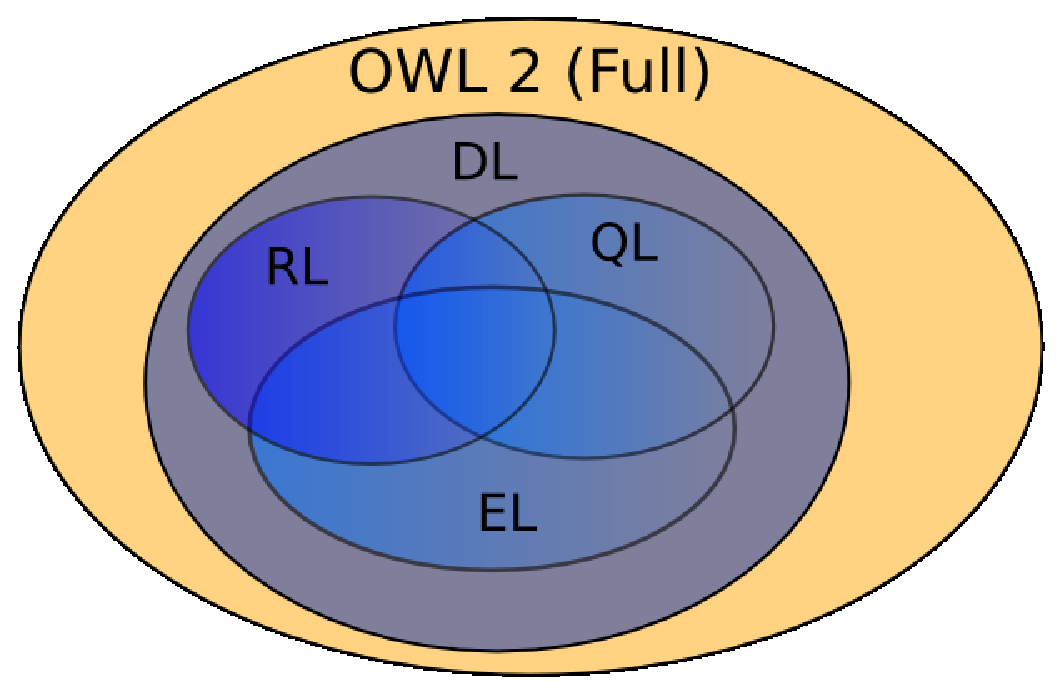
\includegraphics[width=0.8\columnwidth]{figures/owl2Profiles}
\par\end{centering}
\caption{OWL2 Profiles.\label{fig:OWL2-Profiles}}
\end{figure}

\selectlanguage{english}%
\begin{description}
\item [{Full}] \foreignlanguage{brazil}{O perfil }OWL Full\foreignlanguage{brazil}{
é direcionado para usuários que querem a máxima expressividade e a
liberdade sintática do }OWL\foreignlanguage{brazil}{ sem garantia
computacional. É improvável que qualquer motor de raciocínio seja
capaz de suportar completamente cada recurso da }OWL Full\foreignlanguage{brazil}{
\citep{mcguinness2004owl}.}
\selectlanguage{brazil}%
\item [{DL}] O perfil \foreignlanguage{english}{OWL DL} (\foreignlanguage{english}{Description
Logic}) é para aplicações que necessitam de máxima expressividade,
enquanto mantém a computabilidade (todas as conclusões são garantidos
para ser computáveis) e decidibilidade (todas as computações terminarão
em tempo finito) \citep{mcguinness2004owl}. \foreignlanguage{english}{OWL
DL} inclui as construções da linguagem \foreignlanguage{english}{OWL},
mas elas podem ser usadas somente sob certas restrições. 
\item [{EL}] O perfil \foreignlanguage{english}{OWL} 2 EL é baseado na
família EL++ de lógica descritiva (\foreignlanguage{english}{Description}
\foreignlanguage{english}{Logic}), esse perfil é particularmente útil
em aplicações utilizando ontologias que contêm um grande número de
propriedades e/ou classes. Além disso, o \foreignlanguage{english}{OWL}
2 EL utiliza um padrão comum utilizado em ontologias para conceitos
e planejamento, ou seja, a combinação de conjunção e qualidades existenciais.
\selectlanguage{english}%
\item [{QL}] \foreignlanguage{brazil}{O perfil }OWL 2 QL\foreignlanguage{brazil}{
é baseado na família }DL-Lite\foreignlanguage{brazil}{ de lógica descritiva,
esse perfil foi criado para permitir o raciocínio (}reasoning\foreignlanguage{brazil}{)
eficiente com grandes quantidades de dados estruturados de acordo
com esquemas relativamente simples, ele fornece a maioria dos recursos
necessários para capturar modelos conceituais, tais como diagramas
de classe UML, diagramas de entidade/relacionamento, e esquemas de
banco de dados. }
\selectlanguage{brazil}%
\item [{RL}] O perfil \foreignlanguage{english}{OWL 2 RL} é voltado para
aplicações que exigem raciocínio escalável em troca de alguma restrição
de poder expressivo. Ele define um subconjunto sintático de \foreignlanguage{english}{OWL
2} que favorece a implementação utilizando tecnologias baseadas em
regras, esse perfil pode ser utilizado na maioria das construções
\foreignlanguage{english}{OWL 2}, porém, para permitir implementações
baseadas em regras de raciocínio, a forma como essas construções podem
ser usadas em axiomas foi restringida. 
\end{description}
\selectlanguage{brazil}%
A ferramenta para definir ontologias da web semântica recomendada
pela comunidade e usada na presente pesquisa foi Protégé\footnote{Ferramenta e framework Protégé \url{http://protege.stanford.edu/}},
que permite um amplo suporte no processo de definição de ontologias.
\selectlanguage{english}%

\section{Domain Specific Language (DSL)\foreignlanguage{brazil}{ }}

\selectlanguage{brazil}%
Em desenvolvimento de software e engenharia de domínio uma linguagem
de domínio específico, em inglês \foreignlanguage{english}{\emph{Domain-Specific
Language}}\emph{ (DSL)}, é um tipo de linguagem de programação ou
linguagem de especificação, dedicada a um domínio particular de problema
com expressões propiás dos especialistas de aquele domínio.

Um usuário, relacionado com um domínio específico, pode usar uma DSL
sem ter experiência em desenvolvimento de software pois a DSL está
relacionada com seu domínio de trabalho, o autor \citet{fowler2010domain}
diz que programadores instruem o computador no que ele deve fazer,
pois já entendem a maneira dele trabalhar, mas com \foreignlanguage{english}{DSLs}
é feito o inverso: o computador começa a entender o que o programador
(usuário) escreve.

Segundo \citet{Mernik:2005:DDL:1118890.1118892} as vantagens das
DSL em comparação com as linguagens de proposito geral são a expressividade,
facilidade de uso e a integração com o domínio da aplicação. O conceito
não é novo, linguagens de programação de propósito especifico existiram
desde o começo das linguagens de programação, mas o termo tornou-se
padrão devido à ascensão da modelagem de domínio específico, elas
são classificadas em:
\selectlanguage{english}%
\begin{itemize}
\item Domain-Specific Markup Languages\foreignlanguage{brazil}{: são linguagens
de um domínio particular com a particularidade de anotar os dados
para que eles sejam sintaticamente distinguíveis, um exemplo deles
é o }Hypertext Markup Language ((HTML \nomenclature{HTML}{HyperText Markup Language})\foreignlanguage{brazil}{
que permite anotar dados no domínio das paginas web.}
\item Domain-specific modeling languages:\foreignlanguage{brazil}{ são linguagens
que permitem expressar informação, conhecimento o sistemas em uma
estrutura consistente com um conjunto de regras que permitem interpretar
o significado dos componentes modelados, um deste tipo de linguagens
é }Unified Modeling Language\foreignlanguage{brazil}{ (}UML\nomenclature{UML}{Unified Modeling Language }\foreignlanguage{brazil}{)
que permite especificar sistemas software.}
\item Domain-specific programming languages:\foreignlanguage{brazil}{ são
linguagens permitem a programação em alto nível aplicado a um domínio
especifico de conhecimento, um exemplo dele é a linguagem R que permite
a programação de conceitos estatísticos e geração de gráficos }
\end{itemize}
\selectlanguage{brazil}%
No caso do SAD SustenAgro, foi analisado que as ontologias permitem
uma definição detalhada do conhecimento do domínio, más o formato
das ontologias requer que os especialistas em sustentabilidade aprendam
os padrões da Web Semântica descrita neste capitulo, o qual não é
trivial, devido a que precisa um conhecimento profundo de modelagem
em formatos semânticos.

Pelo qual a definição de uma DSL particular para os especialistas
do domínio, permitiria fornecer uma solução compatível com os termos
específicos deles, com o qual seria possível a especialistas especificar
o SAD com um grau de detalhamento suficiente para definir o conhecimento
deles sem intervenção dos desenvolvedores de software, os especialistas
poderiam se tornar, na prática, programadores de seus próprios SADs.

A DSL fará uso e gerenciara a ontologia para organizar o conhecimento
do domínio em um formato compatível com as tecnologias web semântica
e assim definir o SAD SustenAgro, a DSL será uma interface entre o
especialista e a ontologia permitindo fornecer que os especialistas
definam ontologias da web semântica.

\begin{figure}
\begin{centering}
\includegraphics[width=0.8\columnwidth]{\string"figures/DSL Diagram\string".png}
\par\end{centering}
\caption{Camada da DSL \label{fig:Camada-da-DSL}}
\end{figure}


\section{Considerações finais}

Os conceitos apresentados anteriormente foram necessários para o desenvolvimento
da presente pesquisa, demostrando que a web semântica fornece o suporte
tecnológico e teórico suficiente para abordar o desenvolvimento de
sistemas baseados em conhecimento, particularmente as ontologias suportaram
vários aspectos cruciais no desenvolvimento deste projeto, pelo qual
elas foram o foco central da presente pesquisa. 

As DSL auxiliam a definição da ontologia, fornecendo uma linguagem
especifica para o especialista, conseguindo de esta maneira que os
especialistas definam o conhecimento deles no sistema SAD.
